\documentclass[11pt,a4paper]{article}
\usepackage[margin=2.1cm]{geometry}
\usepackage{lmodern}
\renewcommand{\familydefault}{\sfdefault}
\usepackage[T1]{fontenc}
\usepackage{graphicx}
\usepackage{booktabs}
\usepackage{tabularx}
\usepackage{enumitem}
\usepackage{xcolor}
\usepackage{fancyvrb}
\usepackage[most]{tcolorbox}
\usepackage{titlesec}
\usepackage[hidelinks]{hyperref}

\definecolor{ink}{HTML}{1F2328}
\definecolor{muted}{HTML}{59636E}
\definecolor{rule}{HTML}{D0D7DE}
\definecolor{shell}{HTML}{F3F5F7}
\definecolor{say}{HTML}{EAF2FB}
\definecolor{sayline}{HTML}{5189C8}
\definecolor{warn}{HTML}{FBF3E6}
\definecolor{warnline}{HTML}{C9963E}

\color{ink}
\setlength{\parindent}{0pt}
\setlength{\parskip}{6pt}
\setlist{itemsep=2pt,topsep=2pt}
\titleformat{\section}{\Large\bfseries}{\thesection}{0.6em}{}
\titleformat{\subsection}{\large\bfseries}{\thesubsection}{0.6em}{}
\titlespacing*{\section}{0pt}{16pt}{6pt}

% a terminal block: what to type
\newtcblisting{term}{listing only,colback=shell,colframe=rule,boxrule=0.4pt,arc=2pt,
  left=6pt,right=4pt,top=1pt,bottom=1pt,
  listing options={basicstyle=\ttfamily\small,columns=fullflexible,keepspaces=true,showstringspaces=false}}
% what to say to the audience
\newtcolorbox{sayit}{colback=say,colframe=sayline,boxrule=0pt,leftrule=2.5pt,arc=0pt,left=8pt,right=6pt,top=4pt,bottom=4pt,
  fonttitle=\bfseries\small,title={Say},coltitle=sayline,colbacktitle=say,attach title to upper={\ \ }}
% something that can go wrong
\newtcolorbox{careful}{colback=warn,colframe=warnline,boxrule=0pt,leftrule=2.5pt,arc=0pt,left=8pt,right=6pt,top=4pt,bottom=4pt}

\newcommand{\ui}[1]{\textbf{#1}}
\newcommand{\cmd}[1]{\texttt{#1}}

\begin{document}

{\raggedright\Huge\bfseries Demonstrating the live\\placement controller\par}
\vspace{4pt}
{\large\color{muted} A step-by-step guide to showing the testbed, the dashboard and the result to someone who has never seen them}\par
\vspace{2pt}
{\small\color{muted} Latency-Aware Edge Game Server Placement\quad\textbullet\quad Ankam Charan Teja, Aranya Roy, Nikhil Kumar Reddy, Yashvardhan Deep, Akshit Singh\\
\url{https://github.com/ankamteja/latency-aware-edge-game-placement}}\par
\vspace{6pt}
{\color{rule}\hrule}

\section*{What you are showing, in one breath}

Edge placement algorithms choose a node with a latency formula,
\emph{propagation delay + size / bandwidth}. It has a term for distance and
none for load. On a real, small edge node, load is what decides latency: the
nearest node is the fastest until it is crowded, then it is the slowest by
seconds. The demo shows a real game-server testbed, with real bots, where a
controller using that formula leaves players on an overloaded node, and a
controller using a load-aware model learned from measurements moves them
off within seconds. The dashboard only displays; everything is driven from a
terminal, so the audience can see that nothing is scripted behind the page.

\begin{sayit}
``Every edge-placement paper and simulator ranks nodes by distance. We built a
real testbed and measured what that misses. Watch what happens to the nearest
node when players pile onto it, under the standard formula and under ours.''
\end{sayit}

\section{Before the audience arrives (10 minutes)}

\begin{enumerate}[leftmargin=*]
\item \textbf{Plug in the charger and set the power mode to Performance}
  (GNOME: top-right menu, Power Mode). This matters: in Balanced mode every
  node is two to three times slower than the models were fitted on (results
  chapter, section 8.6). Unplugging the charger silently switches it back.
\item \textbf{Close heavy apps} (other browsers, video, builds). The four game
  servers, up to 160 bots and the dashboard share one laptop.
\item \textbf{Bring the testbed up and check it.} After a reboot the container
  links are gone and must be recreated; otherwise only the check is needed:
\begin{term}
cd ~/latency-aware-edge-game-placement
topology/up.sh            # only after a reboot; ends with ALL CHECKS PASSED
topology/verify.sh        # must end with ALL CHECKS PASSED
\end{term}
\item \textbf{Start the dashboard} in its own terminal and leave it running:
\begin{term}
live/run.sh               # prints: dashboard: http://127.0.0.1:8090
\end{term}
\item Open \url{http://127.0.0.1:8090} in a browser, press \cmd{Ctrl+Shift+R}
  once (loads the newest page), and make the window full screen.
\item Open a second terminal next to the browser, large font, in the
  repository folder. This is the one the audience watches you type into.
\end{enumerate}

\begin{careful}
\textbf{Check before you start:} the top strip of the dashboard shows no run,
\ui{Start run} is enabled, and \cmd{topology/verify.sh} passed in the last
few minutes. If a previous session was left running, \cmd{live/load.sh stop}
ends it and disconnects every bot.
\end{careful}

\begin{careful}
\textbf{No testbed available} (another laptop, a projector PC, a viva
online)? Open \url{https://ankamteja.github.io/latency-aware-edge-game-placement/}.
It is the same dashboard playing back the runs recorded on 2026-10-21 from
their logs: pick a controller and a scenario, press \ui{Start run}, choose the
speed (4x keeps a 13-minute run under 4 minutes). Demos 1 to 3 below become
``analytical, standard'', ``learned, standard'' and ``learned, corrected live,
capacity drop''. Say that it is a replay; nothing in it is simulated.
\end{careful}

\section{A tour of the screen (2 minutes)}

\begin{center}
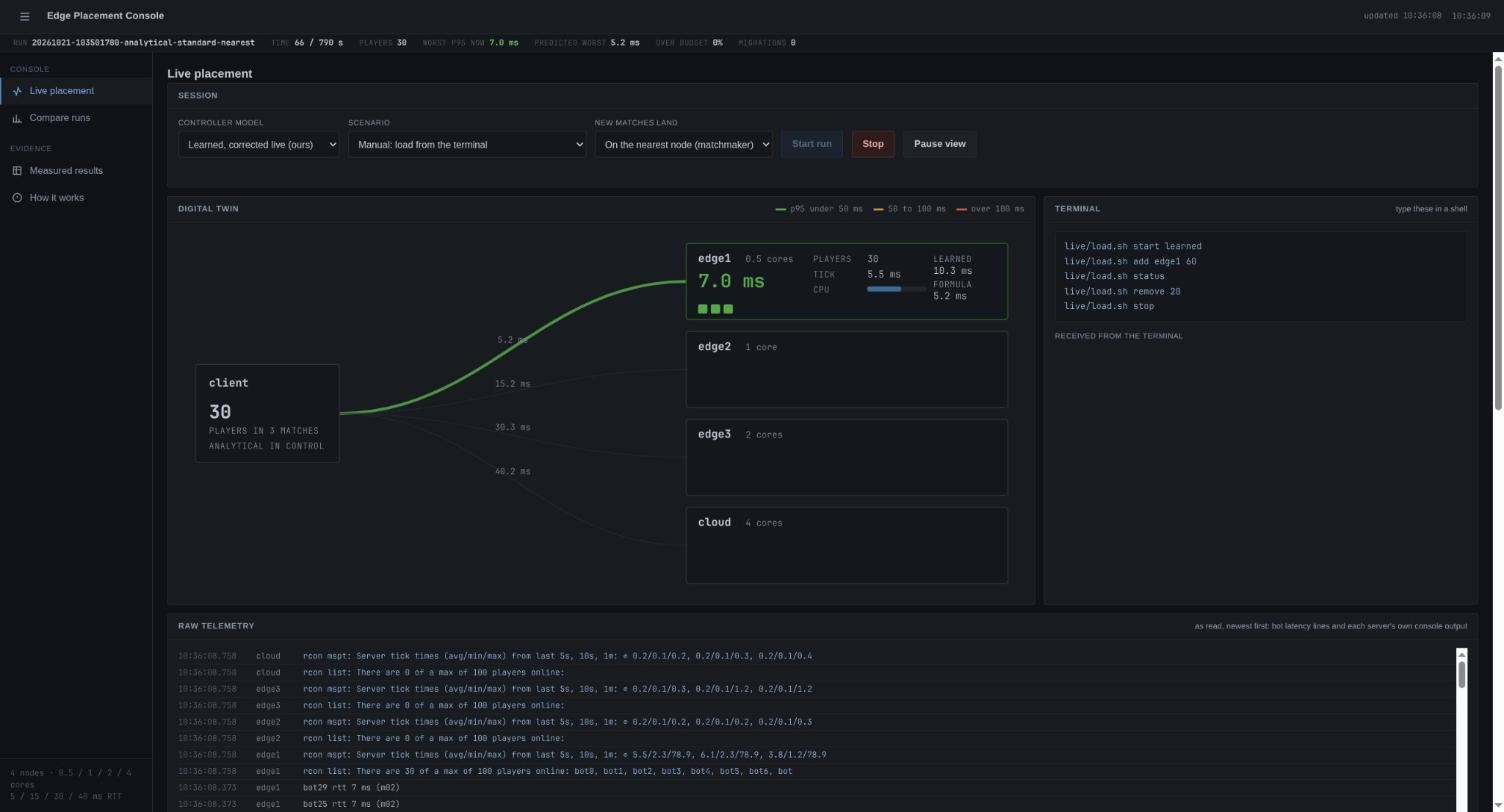
\includegraphics[width=\linewidth]{img/live-top.jpg}
\end{center}

\begin{description}[leftmargin=0pt,style=nextline]
\item[Top strip] the run's name, elapsed time, players connected, the
  \emph{worst} node's measured p95 right now, what the controller
  \emph{predicted} for it, the share of time over the 100 ms budget, and how
  many matches have been moved. The update time on the right turns amber if
  the feed stops.
\item[Session] which model controls placement, the scenario, and where new
  matches land. While a run is going the form shows that run and is locked.
\item[Digital twin] the client on the left, the four servers on the right,
  each line labelled with its measured network delay (5, 15, 30, 40 ms). Each
  server shows players, server tick time, CPU, the measured p95 in large type
  (green under 50 ms, amber 50 to 100, red above 100), what the learned model
  and the formula predict at this load, and one square per match of ten
  players. A moving dot is a match being migrated.
\item[Terminal] the commands you can type, and every command received from
  a terminal, as it arrives.
\item[Raw telemetry] the data itself, newest first: one line per bot latency
  sample (\cmd{bot23 rtt 7 ms (m02)}) and each server's own console answers
  (\cmd{rcon list: There are 40 of a max of 100 players online:}
  followed by the bot names). Point at this when someone asks whether the numbers are real.
\end{description}

\begin{center}
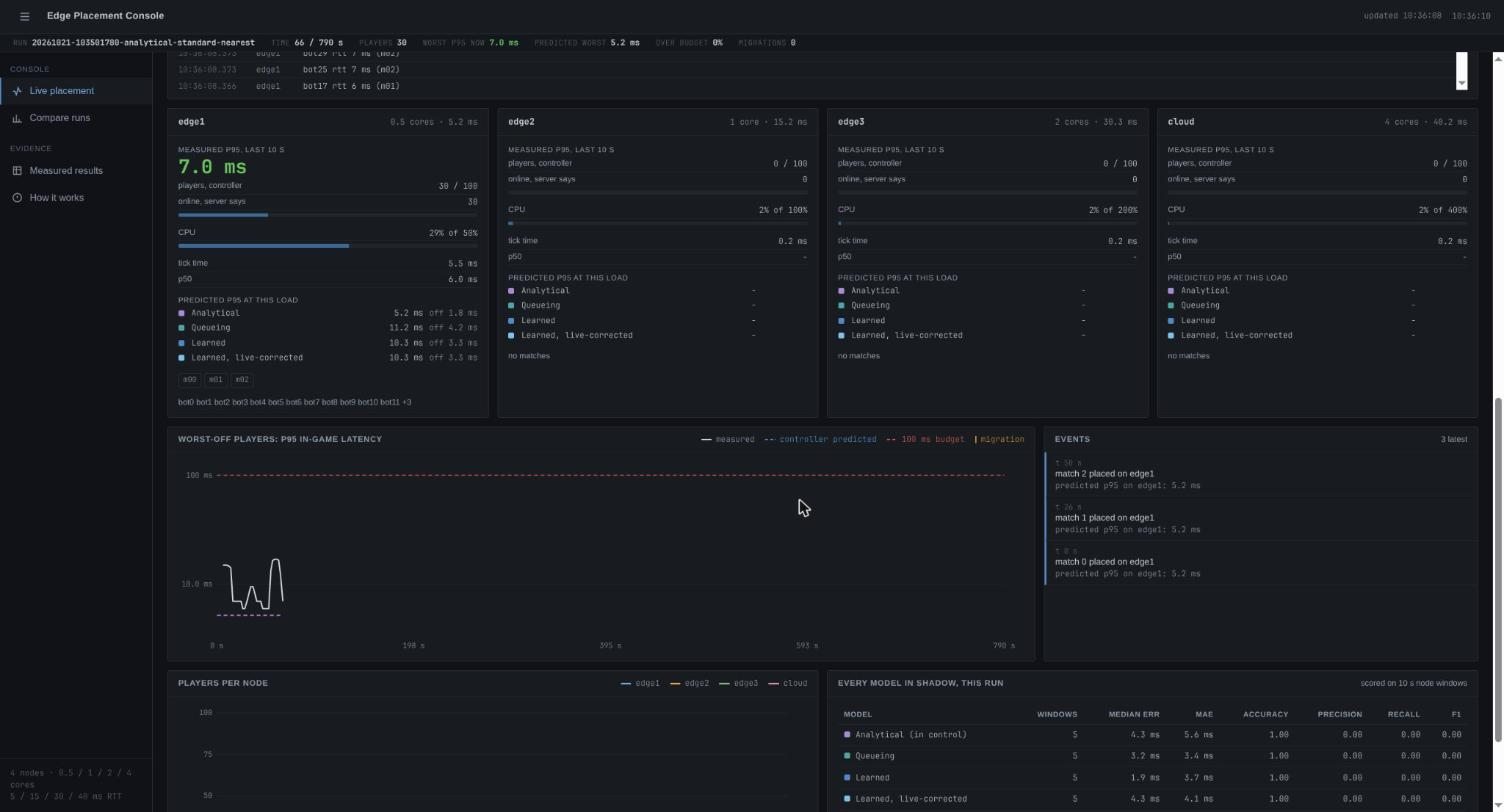
\includegraphics[width=\linewidth]{img/live-bottom.jpg}
\end{center}

Further down: one card per node with the measured p50/p95, the players the
controller placed next to the players the server itself reports, CPU against
the node's quota, and every model's prediction for the node at this load with
how far off it is; the worst-player latency over time with the controller's
prediction and the migrations marked; the event log; players per node over
time; and a table scoring every model in the background on this run's own
measurements (median error, F1 at 50 and 100 ms).

\section{Demo 1: the standard formula leaves players on a crowded node (3 minutes)}

\begin{term}
live/load.sh start analytical     # a terminal-driven session, formula in control
live/load.sh add edge1 60         # 60 real bots straight onto the 0.5-core edge
live/load.sh status               # the twin, as a table
\end{term}

What happens: within one tick edge1 shows 60 players; within seconds its p95
climbs into the seconds and its card turns red. The formula column still says
about 5 ms, because the formula has no load term, so the controller sees no
reason to move anyone. Measured this morning: \textbf{60 players held on edge1,
p95 9.3 s after 95 s, predicted 5 ms, zero migrations}.

\begin{sayit}
``This is the standard model. It predicts 5 milliseconds because edge1 is
5 milliseconds away. The players on it are waiting over 9 seconds. It will
never move them: from its point of view edge1 is still the best node.''
\end{sayit}

\begin{term}
live/load.sh stop
\end{term}

\section{Demo 2: the load-aware controller recovers (4 minutes)}

\begin{term}
live/load.sh start learned-live   # our model, corrected from live measurements
live/load.sh add edge1 60
\end{term}

\begin{center}
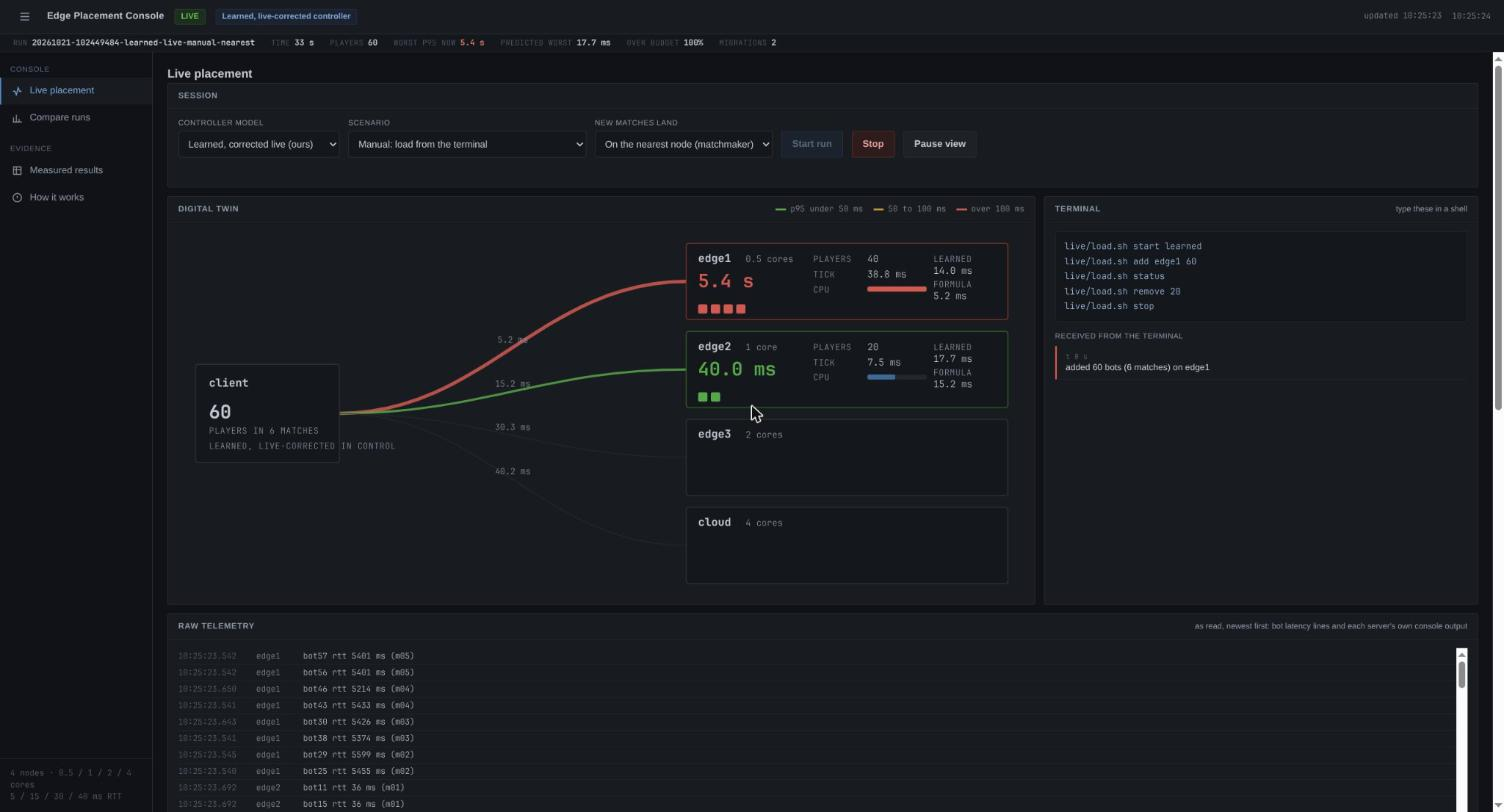
\includegraphics[width=0.92\linewidth]{img/twin-overload.jpg}
\end{center}

What happens: the same overload, but every 10 seconds the controller moves
one match to wherever the predicted worst latency drops most. You see dots
travel from edge1 to edge2 (and edge3), the event log names each move, and
edge1's p95 falls back. Measured this morning: four moves in the first
60 s (edge1 to edge2 at 8, 25 and 40 s, to edge3 at 59 s), the worst node back
under 50 ms by about 70 s and steady near 32 ms after that, then one match
drifting back to edge1 once it was safe.

\begin{sayit}
``Same players, same servers. This controller knows a crowded edge is slow,
because its model was learned from measurements of these servers. It moves
one match at a time, so ten players reconnect each time; you can see each
move in the event log with its predicted gain.''
\end{sayit}

\section{Demo 3: a node gets slower and nobody is told (3 minutes)}

Leave Demo 2 running with about 30 players on edge1, then halve edge1's CPU
from the terminal. No model is told.

\begin{term}
live/load.sh throttle edge1 0.25  # edge1 now has a quarter core instead of half
live/load.sh status
\end{term}

What happens: edge1's p95 jumps; the learned model's offline curve still
predicts a healthy node, but the live-corrected model compares each 10 s window
with its prediction and estimates how much more each player now costs edge1.
In this morning's manual run its estimate rose from 1.1 to about 2.0 within a
minute (the true factor is 2: half the CPU), it moved one match off, and edge1
settled at 14 to 26 ms with 20 players. The twin then shows the cut on edge1's
card in red:

\begin{center}
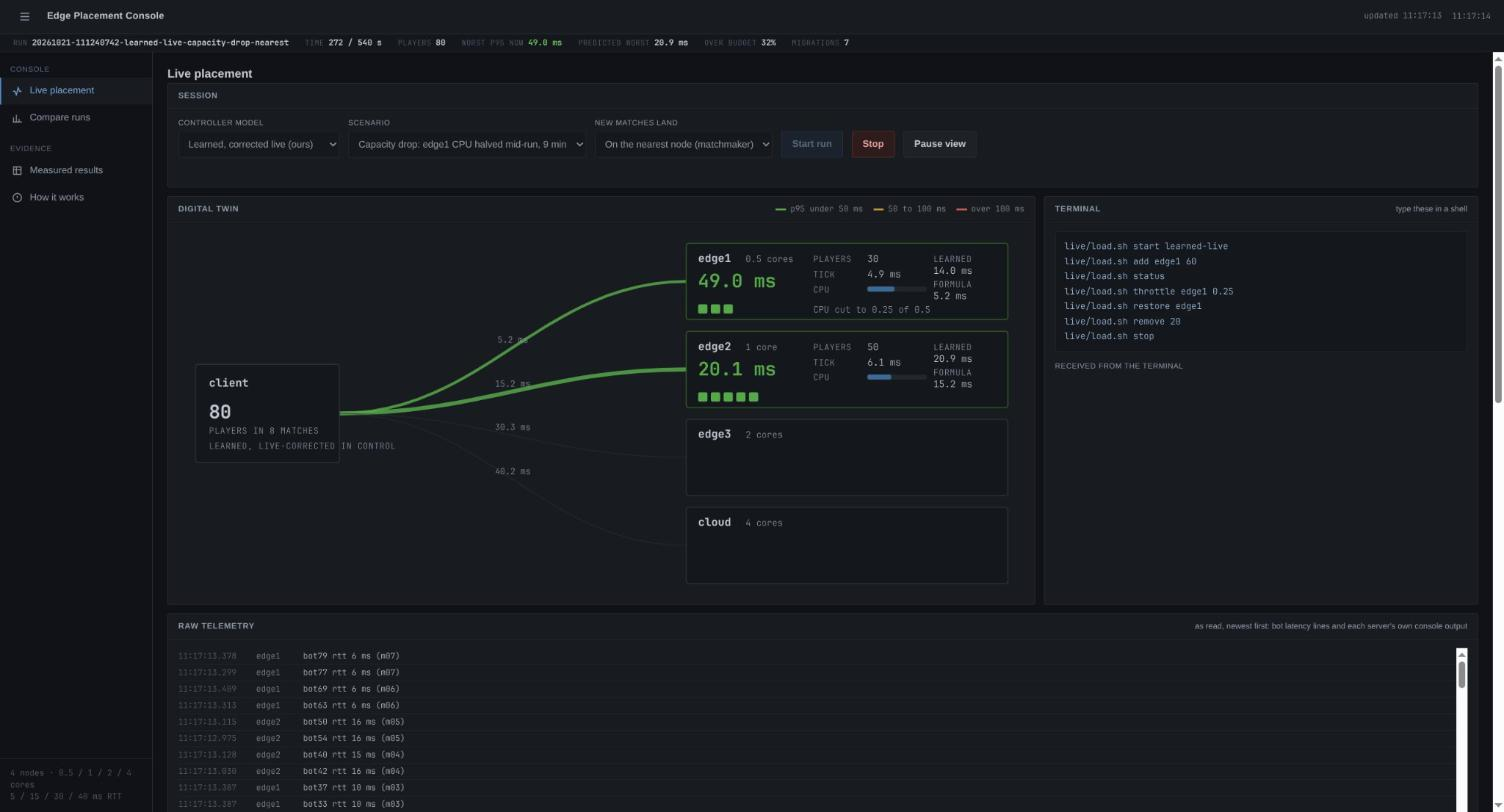
\includegraphics[width=0.92\linewidth]{img/twin-capacity-drop.jpg}
\end{center}

\begin{sayit}
``A noisy neighbour, a throttled host, a smaller VM: the node got slower and
nothing told the controller. It noticed from the measurements alone and
estimated a factor of two, which is exactly what we did to it.''
\end{sayit}

\begin{term}
live/load.sh restore edge1        # give edge1 its CPU back
live/load.sh remove 20            # take two matches off
live/load.sh stop                 # end the session, disconnect every bot
\end{term}

\section{The recorded comparisons (2 minutes)}

Open \ui{Compare runs}. Every finished run is listed with its controller,
worst-player p95 (median and maximum), time over budget, samples over budget,
migrations and the mean reconnect time; tick two runs to overlay their
worst-player latency. The table below is the same comparison measured on a
fixed 13-minute schedule (up to 140 players arriving and leaving the same way
for both), and a 9-minute run in which edge1's CPU is halved at 220 s.

\begin{center}\small
\begin{tabularx}{\linewidth}{@{}Xrrrr@{}}
\toprule
\textbf{Run (2026-10-21), worst node's p95} & \textbf{median} & \textbf{over 100 ms} & \textbf{max} & \textbf{moves} \\
\midrule
Standard, analytical controller & 1\,058 ms & 53\% & 19.6 s & 0 \\
Standard, queueing controller & 166 ms & 53\% & 5.7 s & 11 \\
Standard, learned controller & 33 ms & 18\% & 817 ms & 10 \\
\addlinespace
CPU cut, queueing & 2.6 s & 83\% & 33 s & 4 \\
CPU cut, learned (offline), 2 runs & 0.5, 7.7 s & 74, 82\% & 2.6, 31 s & 4 \\
CPU cut, learned, corrected live, 2 runs & 24, 43 ms & 2, 14\% & 0.2, 4.5 s & 8, 12 \\
\bottomrule
\end{tabularx}
\end{center}
Queueing loads edge2 to 80 players, past its knee; learned stops at 70.
After the CPU cut, queueing and the offline learned model keep 40 players on
the slowed edge1; the live-corrected model takes it down to 20 or fewer within
30 s. Its two runs differ (2\% and 14\%): in the second, its own moves and a
re-probe of edge1 after its memory expired cost the extra time.
The graphs of both comparisons are figures 6 and 7 in the repository's
\texttt{figures/} folder.

\begin{sayit}
``This is the same schedule of players under each controller, recorded on the
testbed, not simulated.''
\end{sayit}

\section{The offline evidence (2 minutes)}

\ui{Measured results} shows the grid behind the models: p95 against players
for every node against what the formula predicts, each model's placement
deployed for real at 40 to 160 players, and every model's out-of-sample
score. The headline: with each model's placement deployed, the worst player's
p95 was 26 / 29\,897 / 17\,758 / 19\,990 ms for the formula at 40 / 80 / 120 /
160 players, and 20 to 39 ms for both load-aware models. \ui{How it works}
is the pipeline on one page: grid, dataset, models, and the live loop.

\section{Questions you will get, and honest answers}

\begin{description}[leftmargin=0pt,style=nextline]
\item[Is this a simulation?] No. Five containers on one laptop: four real
  Minecraft (Paper 1.21.4) servers with real CPU limits and network delay set
  by Linux netem, and real protocol-level bots. The raw telemetry panel shows
  the samples and the servers' own console replies.
\item[Does the learned model place better than queueing theory?] Not on the
  four offline scenarios: a correctly fitted M/M/1 model placed as well. The
  learned model predicts latency best (median error 0.9 ms, 1.2 ms on a
  held-out third replicate, against 1.8 and 2.3 ms). The claim is that the
  load-blind formula fails, by orders of magnitude, and that any load-aware
  model avoids it.
\item[Why is a migration a disconnect?] The controller stops the match on one
  server and starts it on another, so its ten players reconnect (about 6 s on
  average here). A production system would hand game state over first; our
  gap is an upper bound.
\item[Why these core counts and delays?] They were chosen so that the
  trade-off exists. The claim is that an inversion exists, is large, and is
  avoided by a load-aware model; not that edge nodes break at a particular
  player count.
\item[What would change on real hardware?] The knees move; their existence
  does not. Section 8.6 of the results lists every limit: one host, three
  replicates, synthetic players, and the power-mode effect itself, which moved
  edge1's knee threefold with nothing else changed.
\end{description}

\section{If something goes wrong}

\begin{tabularx}{\linewidth}{@{}>{\raggedright\arraybackslash}p{0.34\linewidth}X@{}}
\toprule
\textbf{You see} & \textbf{Do} \\
\midrule
Page does not load & \cmd{live/run.sh} is not running, or failed its check: run \cmd{topology/verify.sh} and read the failed line. \\
\ui{Start run} disabled, ``testbed busy'' & A measurement script is running. Wait for it, or stop it. \\
Update time turns amber & The controller stopped sending. Look at the \cmd{live/run.sh} terminal for an error; restart it. \\
Players stay at 0 after \cmd{add} & Bots cannot join: \cmd{topology/verify.sh}; after a reboot, \cmd{topology/up.sh}. \\
Every node much slower than this guide & Power mode is not Performance, or the charger is unplugged. The run's event log warns about it at start. \\
A node still throttled after a crash & The next run restores it at start; \cmd{topology/verify.sh} reports it. \\
\bottomrule
\end{tabularx}

\section*{Cheat sheet}

\begin{term}
topology/verify.sh                 # ALL CHECKS PASSED
live/run.sh                        # dashboard on http://127.0.0.1:8090
live/load.sh start analytical      # or learned, queueing, learned-live
live/load.sh add edge1 60          # bots in matches of 10
live/load.sh status
live/load.sh throttle edge1 0.25   # node gets slower, no model told
live/load.sh restore edge1
live/load.sh remove 20 [node]
live/load.sh stop
live/ab.sh standard                # formula vs learned, same schedule, ~30 min
\end{term}

\end{document}
